\section{第二章\quad 传输线理论}

\begin{frame}{传输线理论}
 \begin{itemize}
  \item \textbf{传输线理论,一维分布参数电路理论,微波电路设计和计算的理论基础。}
  \item \textbf{传输线理论,电路理论与场的理论之间起着桥梁的作用。}
 \end{itemize}
\end{frame}

\subsection{传输线方程}
\begin{frame}{传输线方程}
 \begin{enumerate}
  \item 传输线的电路模型
 \end{enumerate}
 \centering
 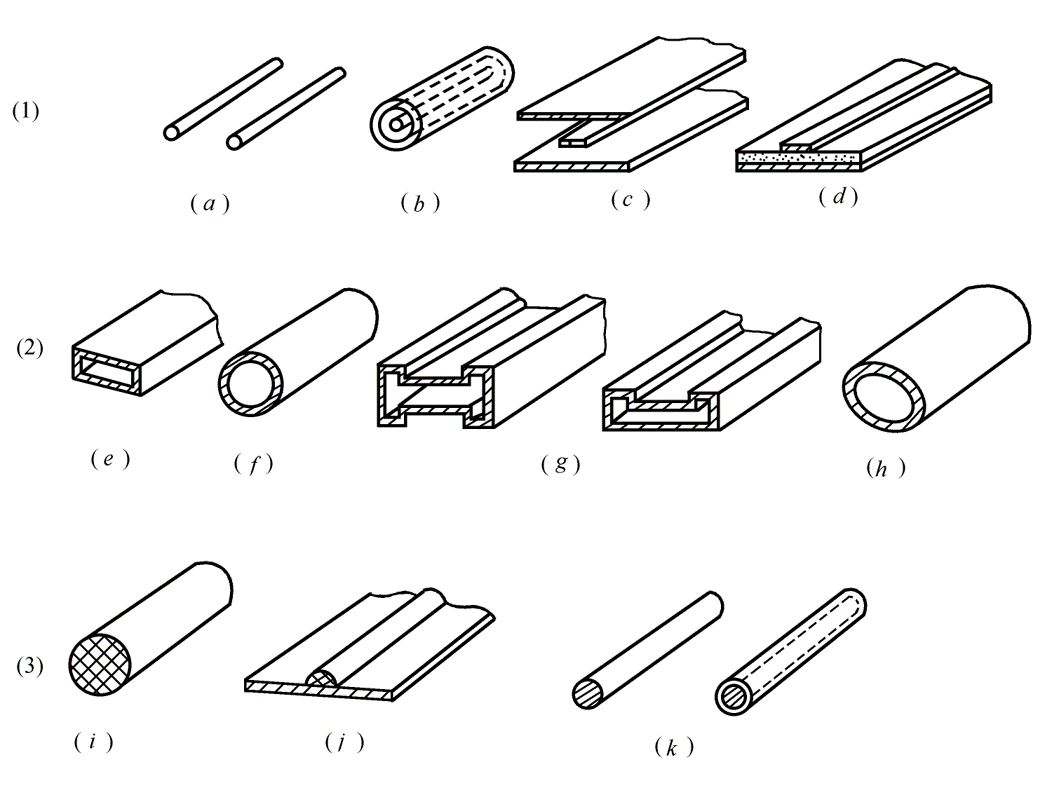
\includegraphics[width=9cm]{guidesystem.png}
 \saveenum
\end{frame}

\begin{frame}{传输线方程}
 \textbf{传输线}是以TEM导模的方式传送电磁波能量或信号的导行系统,其横向尺寸远小于其上工作波长。\\
 \textbf{传输线}有\textbf{长线}和\textbf{短线}之分。所谓长线是指传输线的几何长度与线上传输电磁波的波长比值(电长度)可相比拟,反之称为短线。\\
 \begin{align*}
  \text{长线}\Longrightarrow\text{分布参数电路} \\
  \text{短线}\Longrightarrow\text{集中参数电路} \\
  \text{分界线:}\widefbox{$l/\lambda\geq 0.05$}
 \end{align*}
 当频率提高到微波波段时,这些分布效应不可忽略,所以微波传输线是一种\textbf{分布参数电路}。这导致传输线上的电压和电流是随时间和空间位置而变化的二元函数。
\end{frame}

\begin{frame}{传输线方程}
 根据传输线上的分布参数是否均匀分布,可将其分为均匀传输线和不均匀传输线。我们可以把均匀传输线分割成许多小的微元段$dz(dz<<\lambda)$,这样每个微元段可以看作集中参数电路,用一个$\Gamma$型网络来等效。于是整个传输线可等效成无穷多个$\Gamma$型网络的级联。\\
 \centering
 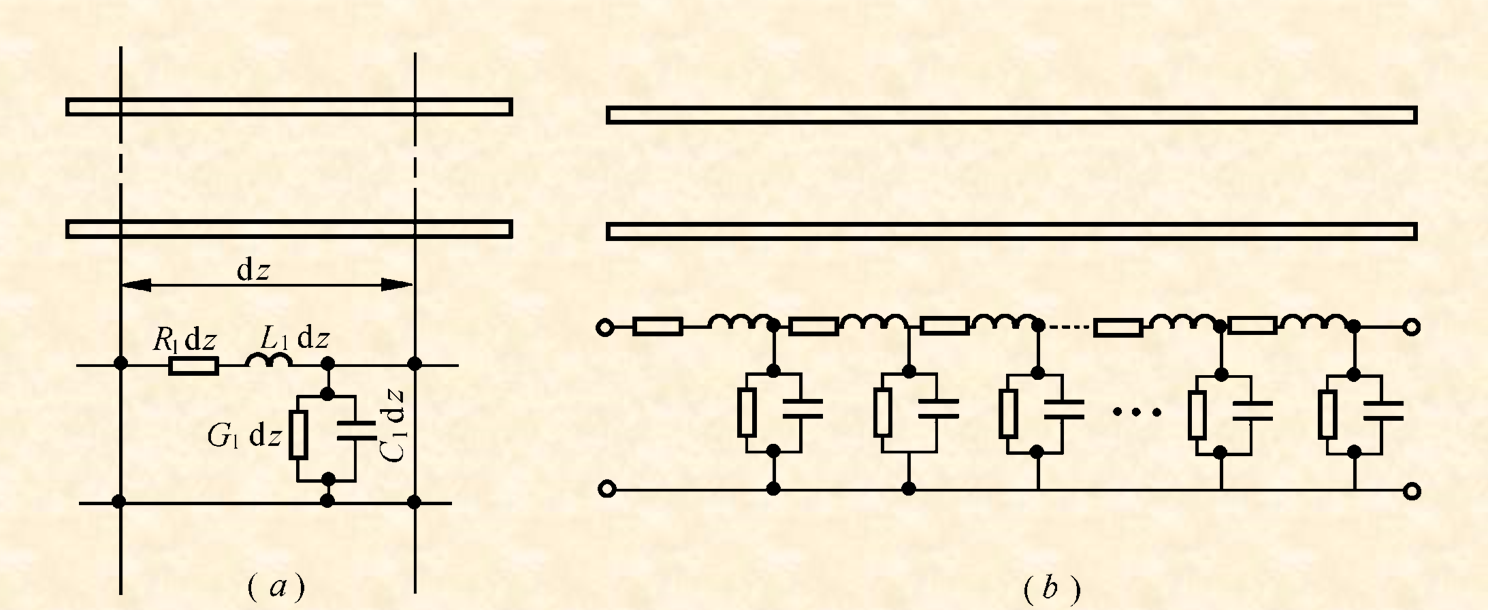
\includegraphics[width=9cm]{transmissionline1.png}
\end{frame}

\begin{frame}{传输线方程}
 双导线、同轴线和平行线传输线的分布参数\\
 \centering
 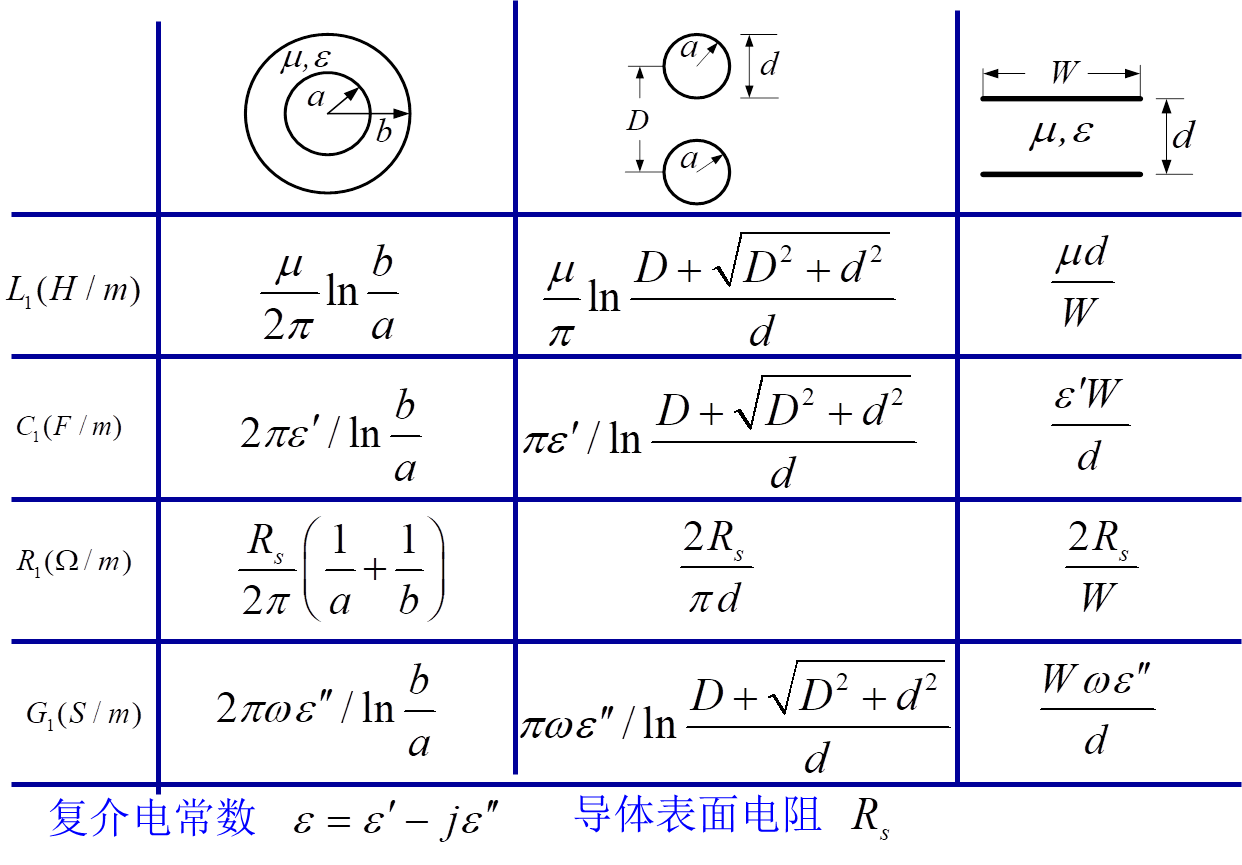
\includegraphics[width=9cm]{tmlineparas.png}
\end{frame}

\begin{frame}{传输线方程}
 \begin{enumerate}
  \resume
  \item 传输线方程\\
        \begin{itemize}
         \item 一般传输线方程或电报方程\\
               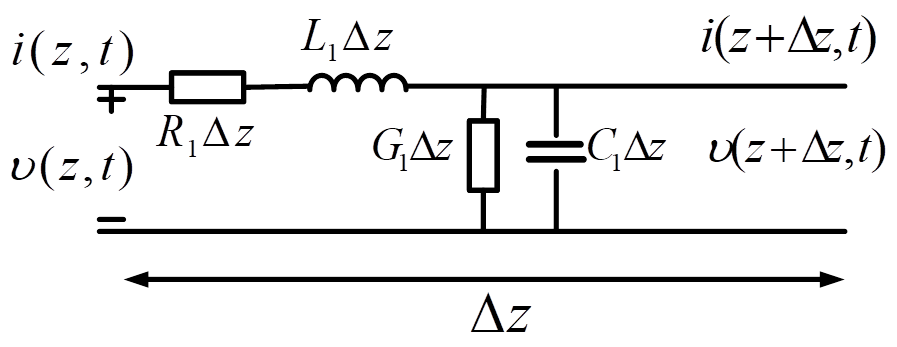
\includegraphics[width=6cm]{transmissionline2.png}
        \end{itemize}
        \saveenum
 \end{enumerate}
 \flushleft
 \fbox{$ v(z+\Delta z,t)=v(z,t)+\frac{\partial v(z,t)}{\partial z}\Delta z $}
 \flushright
 \fbox{$ i(z+\Delta z,t)=i(z,t)+\frac{\partial i(z,t)}{\partial z}\Delta z $}\\
 \begin{align*}
   f(x)=f(x_{0})+f^{'}(x_{0})(x-x_{0})  +\frac{f^{''}(x_{0})}{2!}(x-x_{0})^{2}+\ldots\\
   +\frac{f^{n}(x_{0})}{n!}(x-x_{0})^{n}+R_{n}(x)
 \end{align*}
\end{frame}

\begin{frame}{传输线方程}
  \centering
  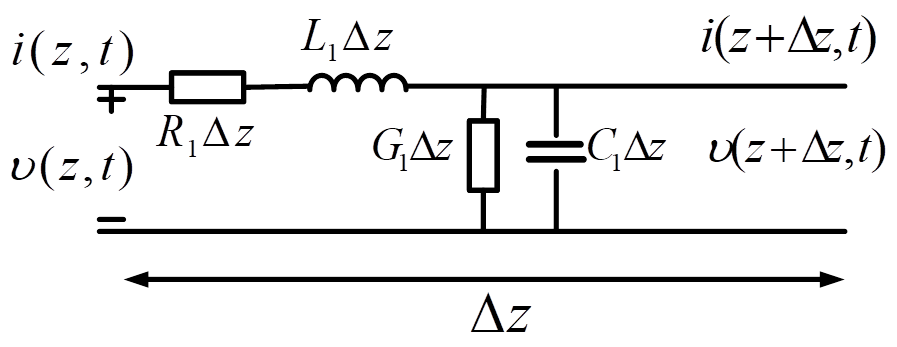
\includegraphics[width=7cm]{transmissionline2.png}
  \flushleft
  线元$\Delta z$上的电压、电流的变化为:
  \begin{empheq}[box=\widefbox]{align*}
    v(z,t)-v(z+\Delta z,t)=-\frac{\partial v(z,t)}{\partial z}\Delta z\\
    i(z,t)-i(z+\Delta z,t)=-\frac{\partial i(z,t)}{\partial z}\Delta z
  \end{empheq}
\end{frame}

\begin{frame}{传输线方程}
  \centering
  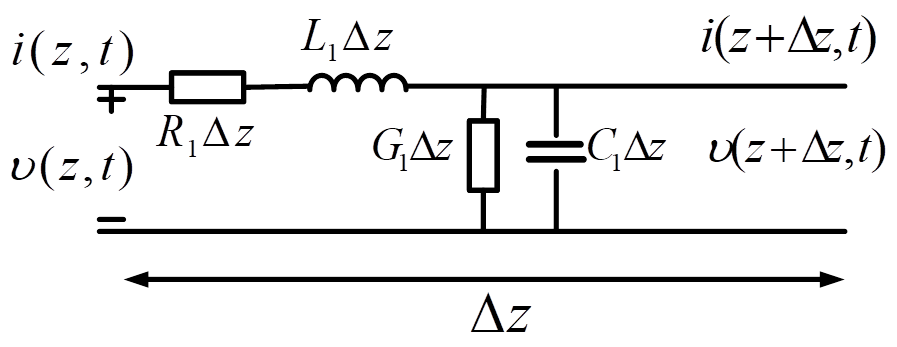
\includegraphics[width=7cm]{transmissionline2.png}
  \flushleft
  线元$\Delta z$上应用基尔霍夫定律,可得:
  \begin{empheq}[box=\widefbox]{align*}
    -\frac{\partial v(z,t)}{\partial z}\Delta z=R_{1}\Delta z\cdot i(z,t)+L_{1}\Delta z\cdot\frac{\partial i(z,t)}{\partial t}\\
    -\frac{\partial i(z,t)}{\partial z}\Delta z=G_{1}\Delta z\cdot v(z,t)+C_{1}\Delta z\cdot\frac{\partial v(z,t)}{\partial t}
  \end{empheq}
\end{frame}

\begin{frame}{传输线方程}
  \begin{empheq}[box=\widefbox]{align*}
    -\frac{\partial v(z,t)}{\partial z}\Delta z=R_{1}\Delta z\cdot i(z,t)+L_{1}\Delta z\cdot\frac{\partial i(z,t)}{\partial t}\\
    -\frac{\partial i(z,t)}{\partial z}\Delta z=G_{1}\Delta z\cdot v(z,t)+C_{1}\Delta z\cdot\frac{\partial v(z,t)}{\partial t}
  \end{empheq}
  \flushleft
  令$\Delta z \rightarrow 0$
  \begin{empheq}[box=\widefbox]{align*}
    \frac{\partial v(z,t)}{\partial z}=-R_{1}\cdot i(z,t)-L_{1}\cdot\frac{\partial i(z,t)}{\partial t}\\
    \frac{\partial i(z,t)}{\partial z}=-G_{1}\cdot v(z,t)-C_{1}\cdot\frac{\partial v(z,t)}{\partial t}
  \end{empheq}
  \centering
  \textbf{一般传输线方程、电报方程}
\end{frame}

\begin{comment}
\newcommand{\mtikzmark}[1]{\tikz[overlay,remember picture]\node(#1){};}
\tikzset{mylabel/.style={align=center,fill=blue!10,font=\footnotesize}}
%\mytlabel[options]{start.mark}{end.mark}{text}
\newcommand\mytlabel[4][]{%
 \tikz[overlay,remember picture]
 {\draw[->]([yshift=-10pt]#2.north) -- node[mylabel,#1]{#4}([yshift=6pt]#3.north);}
}
\end{comment}

\begin{frame}{传输线方程}
  \begin{itemize}
    \item 时谐均匀传输线方程
  \end{itemize}
  \begin{empheq}[box=\widefbox]{align*}
    \frac{\partial v(z,t)}{\partial z}=-R_{1}\cdot i(z,t)-L_{1}\cdot\frac{\partial i(z,t)}{\partial t}\\
    \frac{\partial i(z,t)}{\partial z}=-G_{1}\cdot v(z,t)-C_{1}\cdot\frac{\partial v(z,t)}{\partial t}
  \end{empheq}
  \begin{columns}
    \begin{column}{0.5\linewidth}
      \begin{empheq}[box=\widefbox]{align*}
        v(z,t)=Re\left[V(z)e^{j\omega t}\right]\\
        i(z,t)=Re\left[I(z)e^{j\omega t}\right]
      \end{empheq}
    \end{column}
    \begin{column}{0.5\linewidth}
      分布参数:$R_{1}$,$L_{1}$,$C_{1}$,$G_{1}$不随位置变化
    \end{column}
  \end{columns}
\end{frame}

\begin{frame}{传输线方程}
  \begin{empheq}[box=\widefbox]{align*}
    \frac{dV(z)}{dz}=-(R_{1}+j\omega L_{1})I(z)=-Z_{1}I(z)\\
    Z_{1}=R_{1}+j\omega L_{1} \text{:单位长度串联阻抗}
  \end{empheq}
  \begin{empheq}[box=\widefbox]{align*}
    \frac{dI(z)}{dz}=-(G_{1}+j\omega C_{1})V(z)=-Y_{1}V(z)\\
    Y_{1}=G_{1}+j\omega C_{1} \text{:单位长度并联导纳}
  \end{empheq}
  对$z$再微商
  \begin{align*}
    \frac{d^2}{dz^2}\left\{
    \begin{aligned}
      V(z)\\I(z)
    \end{aligned}
    \right\}-\gamma^2
    \left\{\begin{aligned}
      V(z)\\I(z)
    \end{aligned}\right\}=0
  \end{align*}
  \textbf{电压传播常数}:\fbox{$\gamma=\sqrt{Z_{1}Y_{1}}=\sqrt{(R_{1}+j\omega L_{1})(G_{1}+j\omega C_{1})}$}
\end{frame}

\begin{frame}{传输线方程}
  \begin{itemize}
    \item 时谐传输线方程电压、电流通解
  \end{itemize}
  电压:
  \begin{empheq}[box=\widefbox]{align*}
    V(z)=A_{1}e^{-\gamma z}+A_{2}e^{\gamma z}
  \end{empheq}
  电流:
  \begin{empheq}[box=\widefbox]{align*}
    I(z)=-\frac{1}{R_{1}+j\omega L_{1}}\frac{dV(z)}{dz}=\frac{1}{Z_{0}}(A_{1}e^{-\gamma z}-A_{2}e^{\gamma z})
  \end{empheq}
  $$\gamma=\sqrt{Z_{1}Y_{1}}=\sqrt{(R_{1}+j\omega L_{1})(G_{1}+j\omega C_{1})}$$
  \textbf{特性阻抗}:
  \begin{empheq}[box=\widefbox]{align*}
    Z_{0}=\sqrt{\frac{R_{1}+j\omega L_{1}}{G_{1}+j\omega C_{1}}}
  \end{empheq}
\end{frame}

\begin{frame}{传输线方程}
  \begin{itemize}
    \item 传输线方程的边界条件和解
  \end{itemize}
  \begin{columns}
    \begin{column}{0.35\linewidth}
      端接条件确定常数:\\
      终端条件\\
      始端条件\\
      信号源和负载条件
    \end{column}
    \begin{column}{0.65\linewidth}
      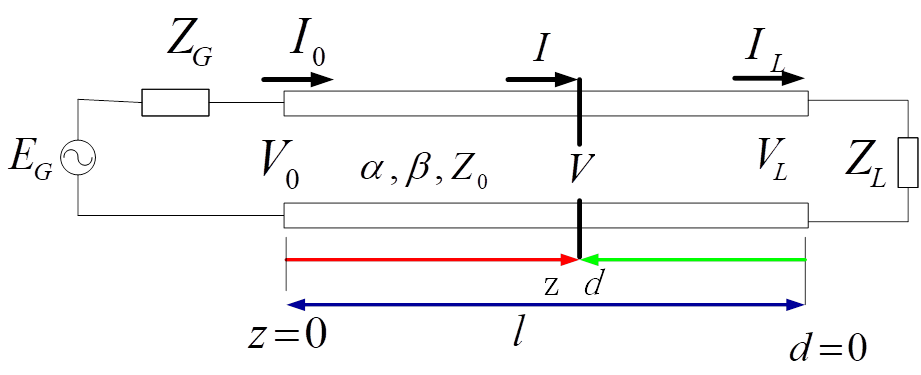
\includegraphics[width=6cm]{tmlineboundary.png}
    \end{column}
  \end{columns}
  \textbf{终端条件}解:
  \begin{columns}
    \begin{column}{0.5\linewidth}
      \begin{empheq}[box=\widefbox]{align*}
        V(z)=A_{1}e^{-\gamma z}+A_{2}e^{\gamma z}
      \end{empheq}
    \end{column}
    \begin{column}{0.5\linewidth}
      \begin{empheq}[box=\widefbox]{align*}
        I(z)=(A_{1}e^{-\gamma z}-A_{2}e^{\gamma z})/Z_{0}
      \end{empheq}
    \end{column}
  \end{columns}
  \begin{empheq}[box=\widefbox]{align*}
    V(l)=V_{L}=A_{1}e^{-\gamma l}+A_{2}e^{\gamma l}\\
    I(l)=I_{L}=\frac{1}{Z_{0}}(A_{1}e^{-\gamma l}-A_{2}e^{\gamma l})
  \end{empheq}
\end{frame}

\begin{frame}{传输线方程}
  \begin{empheq}[box=\widefbox]{align*}
    A_{1}=\frac{V_{L}+I_{L}Z_{0}}{2}e^{\gamma l},A_{2}=\frac{V_{L}-I_{L}Z_{0}}{2}e^{-\gamma l}
  \end{empheq}
  代入:
  \begin{columns}
    \begin{column}{0.45\linewidth}
      \begin{empheq}[box=\widefbox]{align*}
        V(z)=A_{1}e^{-\gamma z}+A_{2}e^{\gamma z}
      \end{empheq}
    \end{column}
    \begin{column}{0.45\linewidth}
      \begin{empheq}[box=\widefbox]{align*}
        I(z)=(A_{1}e^{-\gamma z}-A_{2}e^{\gamma z})/Z_{0}
      \end{empheq}
    \end{column}
  \end{columns}
  对于终端边界条件场合,我们常采用$d$(终端出发)坐标系$d$,换坐标\fbox{$d=l-z$}
  \begin{empheq}[box=\widefbox]{align*}
    V(d)=\frac{V_{L}+I_{L}Z_{0}}{2}e^{\gamma d}+\frac{V_{L}-I_{L}Z_{0}}{2}e^{-\gamma d}=V^{+}(d)+V^{-}(d)\\
    I(d)=\frac{V_{L}+I_{L}Z_{0}}{2Z_{0}}e^{\gamma d}-\frac{V_{L}-I_{L}Z_{0}}{2Z_{0}}e^{-\gamma d}=I^{+}(d)+I^{-}(d)
  \end{empheq}
\end{frame}

\begin{frame}{传输线方程}
  \begin{empheq}[box=\widefbox]{align*}
    V(d)=\frac{V_{L}+I_{L}Z_{0}}{2}e^{\gamma d}+\frac{V_{L}-I_{L}Z_{0}}{2}e^{-\gamma d}=V^{+}(d)+V^{-}(d)\\
    I(d)=\frac{V_{L}+I_{L}Z_{0}}{2Z_{0}}e^{\gamma d}-\frac{V_{L}-I_{L}Z_{0}}{2Z_{0}}e^{-\gamma d}=I^{+}(d)+I^{-}(d)
  \end{empheq}
  \begin{empheq}[box=\widefbox]{align*}
    V(d)=\frac{e^{\gamma d}+e^{-\gamma d}}{2}V_{L}+\frac{e^{\gamma d}-e^{-\gamma d}}{2}Z_{0}I_{L}\\
    I(d)=\frac{e^{\gamma d}+e^{-\gamma d}}{2}\frac{1}{Z_{0}}V_{L}+\frac{e^{\gamma d}-e^{-\gamma d}}{2}I_{L}
  \end{empheq}
  \begin{align*}
    \begin{bmatrix}
      V(d)\\I(d)
    \end{bmatrix}
    =
    \begin{bmatrix}
      \cosh\gamma d & Z_{0}\sinh\gamma d\\
      Z_{0}^{-1}\sinh\gamma d & \cosh\gamma d
    \end{bmatrix}
    \begin{bmatrix}
      V_{L}\\I_{L}
    \end{bmatrix}
  \end{align*}
\end{frame}

\begin{frame}{传输线方程}
  \textbf{始端条件解}:已知始端电压和电流$V_{0},I_{0}$ \\
  \fbox{$V(z)=A_{1}e^{-\gamma z}+A_{2}e^{\gamma z}$}
  \fbox{$I(z)=(A_{1}e^{-\gamma z}-A_{2}e^{\gamma z})/Z_{0}$}\\
  \begin{columns}
    \begin{column}{0.3\linewidth}
      \begin{align*}
        V_{0}=A_{1}+A_{2}\\
        I_{0}=(A_{1}-A_{2})/Z_{0}
      \end{align*}
    \end{column}
    \begin{column}{0.1\linewidth}
      \centering
      $ \longrightarrow $
    \end{column}
    \begin{column}{0.6\linewidth}
      \begin{empheq}[box=\fbox]{align*}
        A_{1}=\frac{V_{0}+I_{0}Z_{0}}{2}\quad A_{2}=\frac{V_{0}-I_{0}Z_{0}}{2}
      \end{empheq}
    \end{column}
  \end{columns}
  \begin{empheq}[box=\widefbox]{align*}
    V(z)=\frac{V_{0}+I_{0}Z_{0}}{2}e^{-\gamma z}+\frac{V_{0}-I_{0}Z_{0}}{2}e^{\gamma z}\\
    I(z)=\frac{V_{0}+I_{0}Z_{0}}{2Z_{0}}e^{-\gamma z}+\frac{V_{0}-I_{0}Z_{0}}{2Z_{0}}e^{\gamma z}
  \end{empheq}
  \begin{align*}
    \begin{bmatrix}
      V(z)\\I(z)
    \end{bmatrix}
    =
    \begin{bmatrix}
      \cosh\gamma z & -Z_{0}\sinh\gamma z\\
      -Z_{0}^{-1}\sinh\gamma z & \cosh\gamma z
    \end{bmatrix}
    \begin{bmatrix}
      V_{0}\\I_{0}
    \end{bmatrix}
  \end{align*}
\end{frame}

\begin{frame}{传输线方程}
  \textbf{信号源和负载条件解}:
  已知信号源电动势 $E_{G}$、
  内阻抗 $Z_{G}$、
  负载阻抗 $Z_{L}$
  \begin{empheq}[box=\widefbox]{align*}
    V(d)=\frac{E_{G}Z_{0}}{Z_{G}+Z_{0}}\cdot\frac{e^{-\gamma l}}{1-\Gamma_{L}\Gamma_{G}e^{-2\gamma l}}(e^{\gamma d}+\Gamma_{L}e^{-\gamma d})\\
    I(d)=\frac{E_{G}}{Z_{G}+Z_{0}}\cdot\frac{e^{-\gamma l}}{1-\Gamma_{L}\Gamma_{G}e^{-2\gamma l}}(e^{\gamma d}-\Gamma_{L}e^{-\gamma d})
  \end{empheq}
  \begin{align*}
    \Gamma_{L}=\frac{Z_{L}-Z_{0}}{Z_{L}+Z_{0}}\quad \Gamma_{G}=\frac{Z_{G}-Z_{0}}{Z_{G}+Z_{0}}\quad\text{反射系数}
  \end{align*}
\end{frame}

\begin{frame}{传输线方程}
  \begin{enumerate}
    \resume
    \item \textbf{传输线的特性参数}
    \begin{itemize}
      \item 特性阻抗
    \end{itemize}
    \begin{align*}
      Z_{0}=\sqrt{\frac{R_{1}+j\omega L_{1}}{G_{1}+j\omega C_{1}}}
    \end{align*}
    传输线上\textbf{行波}的电压与电流之比称为传输线的特性阻抗\\
    $$\text{无耗线}R_{1}=G_{1}=0\quad Z_{0}=\sqrt{\frac{L_{1}}{C_{1}}}$$\\
    微波低耗线$R_{1}<<\omega L_{1},G_{1}<<\omega C_{1}$\\
    $$Z_{0}=\sqrt{\frac{R_{1}+j\omega L_{1}}{G_{1}+j\omega C_{1}}}\approx\sqrt{\frac{L_{1}}{C_{1}}}\left[1+\frac{1}{2}\left(\frac{R_{1}}{j\omega L_{1}}-\frac{G_{1}}{j\omega C_{1}}\right)\right]$$
  \end{enumerate}
\end{frame}

\begin{frame}{传输线方程}
  \begin{itemize}
    \item \textbf{双导线特性阻抗}\\
    $$Z_{0}=120\ln\left[\frac{D}{d}+\sqrt{\left(\frac{D}{d}\right)^{2}-1}\right]$$
    \item \textbf{同轴线特性阻抗}\\
    $$Z_{0}=\frac{60}{\sqrt{\epsilon_{r}}}\ln\frac{b}{a}$$
    \item \textbf{平行板传输线特性阻抗}\\
    $$Z_{0}=\frac{d}{W}\eta$$
  \end{itemize}
\end{frame}

\begin{frame}{传输线方程}
  \begin{itemize}
    \item \textbf{传播常数}
  \end{itemize}
  描述导行波沿着导行系统传播过程中的\textbf{衰减和相位变化}的参数
  \begin{empheq}[box=\widefbox]{align*}
    \gamma = \sqrt{(R_{1}+j\omega L_{1})(G_{1}+j\omega C_{1})}=\alpha+j\beta
  \end{empheq}
  $\alpha$——衰减常数,单位$Np/m$或$dB/m$\quad $(1Np=8.686dB)$\\
  $\beta$——相位常数,单位$rad/m$\\
  \centering
  $\text{无耗线}\quad \alpha=0$\quad \fbox{$\beta=\omega\sqrt{L_{1}C_{1}}$}
\end{frame}

\begin{frame}{传输线方程}
  微波低耗线\quad$R_{1}<<\omega L_{1},G_{1}<<\omega C_{1}$
  \begin{align*}
    \gamma &=\sqrt{(R_{1}+j\omega L_{1})(G_{1}+j\omega C_{1})}=\alpha+j\beta\\
           &=\sqrt{(j\omega)^{2}L_{1}C_{1}}\sqrt{\left(1+\frac{R_{1}}{j\omega L_{1}}\right)(1+\frac{G_{1}}{j\omega C_{1}})}\\
           &\approx\frac{1}{2}\left(R_{1}\sqrt{C_{1}/L_{1}}+G_{1}\sqrt{L_{1}/C_{1}}\right)+j\omega\sqrt{L_{1}C_{1}}
  \end{align*}
  \begin{columns}
    \begin{column}{0.65\linewidth}
      \begin{empheq}[box=\widefbox]{align*}
        \therefore\alpha=\frac{R_{1}}{2Z_{0}}+\frac{G_{1}Z_{0}}{2}=\alpha_{c}+\alpha_{d}
      \end{empheq}
      $\alpha_{c}$:分布电阻产生的导体衰减常数\\
      $\alpha_{d}$:漏电导产生的介质衰减常数
    \end{column}
    \begin{column}{0.35\linewidth}
      \begin{empheq}[box=\widefbox]{align*}
        \therefore\beta=\omega\sqrt{L_{1}C_{1}}
      \end{empheq}
      $\beta$:近似于无耗传输线的相位常数
    \end{column}
  \end{columns}
\end{frame}

\begin{frame}{传输线方程}
  对于TEM导波:\\
  $$k_{c}=0,\lambda_{c}=\infty$$\\
  其相速度为\\
  $$v_{p}=v=\frac{\omega}{\beta}=\frac{1}{\sqrt{L_{1}C_{1}}}$$\\
  波长为\\
  $$\lambda_{g}=\lambda=\frac{2\pi}{\beta}=\frac{v_{p}}{f}$$\\
  特性阻抗为\\
  $$Z_{0}=\sqrt{\frac{L_{1}}{C_{1}}}=\frac{1}{v_{p}C_{1}}=v_{p}L_{1}$$\\
  \textbf{传输线的特性阻抗可由单位长度分布电容或分布电感求得}
\end{frame}

\subsection{分布参数阻抗}
\begin{frame}{分布参数阻抗}
  \begin{itemize}
    \item 微波阻抗——由微波传输线上的电压和电流决定的,是\textbf{分布参数}阻抗。(低频传输线阻抗是\textbf{集中参数}阻抗)
    \item 微波阻抗——与导行系统上导波的反射或者驻波特性密切相关,即与导行系统的状态或者特性密切相关。
    \item 微波阻抗不能直接测量,需要借助反射参量或者驻波参量的直接测量而间接获得。
  \end{itemize}
\end{frame}

\begin{frame}{分布参数阻抗}
  \begin{enumerate}
    \item \textbf{分布参数阻抗}
    \saveenum
  \end{enumerate}
  \centering
  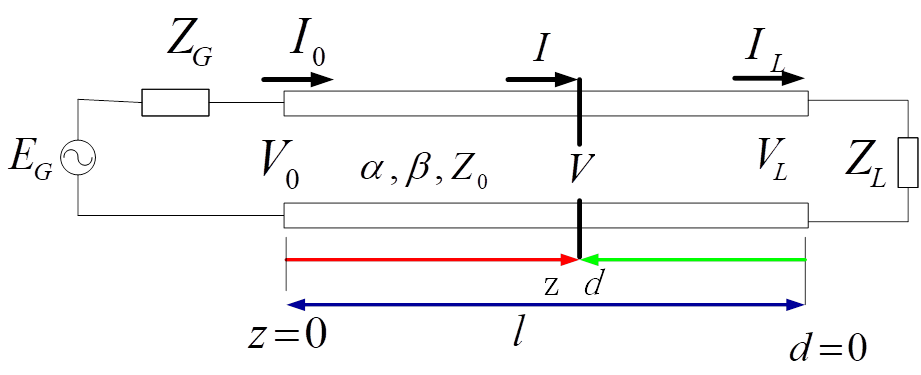
\includegraphics[width=8cm]{tmlineboundary.png}
  \begin{align*}
    \begin{bmatrix}
      V(d)\\I(d)
    \end{bmatrix}=
    \begin{bmatrix}
      \cosh\gamma d\quad Z_{0}\sinh\gamma d\\
      Z_{0}^{-1}\sinh\gamma d\quad \cosh\gamma d
    \end{bmatrix}
    \begin{bmatrix}
      V_{L}\\I_{L}
    \end{bmatrix}
  \end{align*}
  \flushleft
  传输线终端接负载阻抗$Z_{L}$时,距离终端$d$处向负载方向看去的输入阻抗定义为该处的电压$V(z)$与电流$I(z)$之比,即
\end{frame}

\begin{frame}{分布参数阻抗}
  \begin{empheq}[box=\widefbox]{align*}
    Z_{in}(d)=\frac{V_{L}\cosh\gamma d+I_{L}Z_{0}\sinh\gamma d}{I_{L}\cosh\gamma d+\frac{V_{L}\sin\beta d}{Z_{0}}}=Z_{0}\frac{Z_{L}+Z_{0}\tanh\gamma d}{Z_{0}+Z_{L}\tanh\gamma d}
  \end{empheq}
  \flushleft
  均匀无耗传输线\\
  $$\alpha=0,\gamma=j\beta,\tanh\gamma d=\tanh(j\beta d)=j\tan\beta d$$
  \begin{columns}
    \begin{column}{0.4\linewidth}
      传输线的阻抗(从$d$点向负载看的输入阻抗,或视在阻抗)
    \end{column}
    \begin{column}{0.6\linewidth}
      \begin{empheq}[box=\widefbox]{align*}
        Z_{in}(d)=Z_{0}\frac{Z_{L}+jZ_{0}\tan\beta d}{Z_{0}+jZ_{L}\tan\beta d}
      \end{empheq}
    \end{column}
  \end{columns}
  \flushleft
  对给定的传输线和负载阻抗,线上各点的输入阻抗随至终端的距离$d$的不同而作周期(周期为$\lambda/2$)变化,是一种\textbf{分布参数阻抗}。它不能直接测量。
\end{frame}

\begin{frame}{分布参数阻抗}
  \flushleft
  均匀无耗传输线\\
  \begin{empheq}[box=\widefbox]{align*}
    Z_{in}(d)=Z_{0}\frac{Z_{L}+jZ_{0}\tan\beta d}{Z_{0}+jZ_{L}\tan\beta d}
  \end{empheq}
  \begin{itemize}
    \item 传输线阻抗,随位置$d$而变,分布于沿线各点,且与负载有关,是一种分布参数阻抗(Distributed Impedance)。由于微波频率下,电压与电流缺乏明确的物理意义,不能直接测量,故传输线阻抗也不能直接测量。
    \item 传输线阻抗具有阻抗变换作用,$Z_{L}$通过线段$d$变换成$Z_{in}(d)$。
    \item 传输线阻抗呈现周期性变化。
  \end{itemize}
\end{frame}

\begin{frame}{分布参数阻抗}
  \flushleft
  在一些特殊位置点上,有如下简单阻抗关系:
  \begin{empheq}[box=\widefbox]{align*}
    & Z_{in}(l)=Z_{L}\qquad l=n\frac{\lambda}{2}(n=0,1,2,\ldots)\\
    & Z_{in}(l)=\frac{Z_{0}^{2}}{Z_{L}}\qquad l=(2n+1)\frac{\lambda}{4}(n=0,1,2,\ldots)
  \end{empheq}
  \begin{itemize}
    \item 传输线上距负载为半波长整数倍的各点输入阻抗等于负载阻抗;\textbf{半波长的重复性}
    \item 距负载为四分之一波长奇数倍的各点输入阻抗等于特性阻抗的平方与负载阻抗的比值
    \item 当$Z_{0}$为实数,$Z_{L}$为复数负载时,四分之一波长的传输线具有变换阻抗性质的作用。\textbf{四分之一波长变换性}
  \end{itemize}
\end{frame}

\begin{frame}
  \flushleft
  在许多情况下,例如并联电路的阻抗计算,采用导纳比较方便:
  \begin{empheq}[box=\widefbox]{align*}
    Y_{in}(d)=\frac{1}{Z_{in}(d)}=Y_{0}\frac{Y_{L}+jY_{0}\tan\beta d}{Y_{0}+jY_{L}\tan\beta d}
  \end{empheq}
\end{frame}

\begin{frame}{反射参量}
  \begin{enumerate}
    \resume
    \item 反射参量
    \saveenum
  \end{enumerate}
  \begin{empheq}[box=\widefbox]{align*}
    V(d)=\frac{V_{L}+I_{L}Z_{0}}{2}e^{\gamma d}+\frac{V_{L}-I_{L}Z_{0}}{2}e^{-\gamma d}
  \end{empheq}
  \begin{itemize}
    \item 反射系数(Reflection Coefficient)
  \end{itemize}
  距终端$d$处的反射波电压$V^{-}(d)$与入射波电压$V^{+}(d)$之比定义为该处的\textbf{电压反射系数}$\Gamma_{v}(d)$,即
  \begin{align*}
    \Gamma_{v}(d)&=\frac{V^{-}(d)}{V^{+}(d)}=\frac{A_{2}e^{-\gamma d}}{A_{1}e^{\gamma d}}\\
                 &=\frac{V_{L}-I_{L}Z_{0}}{V_{L}+I_{L}Z_{0}}e^{-2\gamma d}=\frac{Z_{L}-Z_{0}}{Z_{L}+Z_{0}}e^{-2\gamma d}
  \end{align*}
\end{frame}

\begin{frame}{反射参量}
  \begin{columns}
    \begin{column}{0.35\linewidth}
      电流反射系数
    \end{column}
    \begin{column}{0.65\linewidth}
      \begin{empheq}[box=\widefbox]{align*}
        I(d)=\frac{V_{L}+I_{L}Z_{0}}{2Z_{0}}e^{\gamma d}-\frac{V_{L}-I_{L}Z_{0}}{2Z_{0}}e^{-\gamma d}
      \end{empheq}
    \end{column}
  \end{columns}
  \begin{align*}
    \Gamma_{I}(d)=\frac{I^{-}(d)}{I^{+}(d)}=-\frac{A_{2}}{A_{1}}e^{-2\gamma d}=-\Gamma_{V}(d)
  \end{align*}
  终端反射系数
  \begin{columns}
    \begin{column}{0.45\linewidth}
      \begin{align*}
        &\Gamma_{L}=\frac{A_{2}}{A_{1}}=\frac{Z_{L}-Z_{0}}{Z_{L}+Z_{0}}\\
        &=\left\lvert\frac{Z_{L}-Z_{0}}{Z_{L}+Z_{0}}\right\rvert e^{j\Phi_{L}}=\lvert\Gamma_{L}\rvert e^{j\Phi_{L}}
      \end{align*}
    \end{column}
    \begin{column}{0.45\linewidth}
      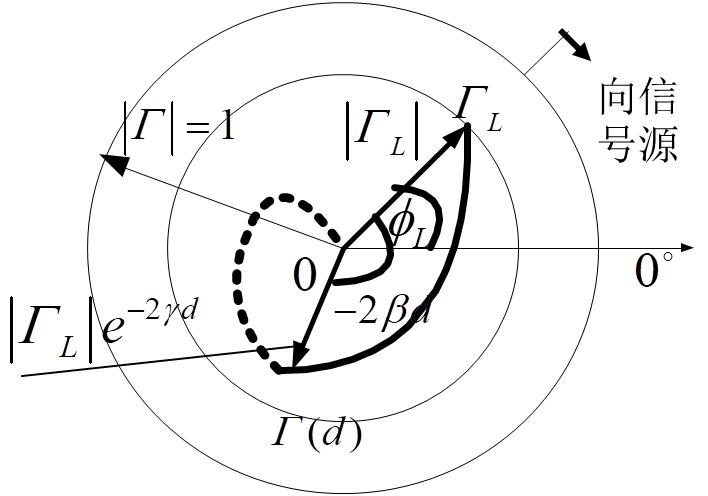
\includegraphics[width=4cm]{chart1.png}
    \end{column}
  \end{columns}
  $$\Gamma(d)=\Gamma_{L}e^{-2\gamma d}\text{传输线上任一点反射系数与终端反射系数的关系}$$
\end{frame}

\begin{frame}{反射参量}
  无耗线情况
  \begin{empheq}[box=\widefbox]{align*}
    \Gamma(d)=\Gamma_{L}e^{-j2\beta d}=\lvert\Gamma_{L}\rvert e^{j(\Phi_{L}-2\beta d)}
  \end{empheq}
  \begin{columns}
    \begin{column}{0.5\linewidth}
      $\Gamma(d)$的大小和相位均在单位圆内,大小不变,相位以$-2\beta d$的角度沿等圆周向信号源(顺时针)方向变化。
    \end{column}
    \begin{column}{0.5\linewidth}
      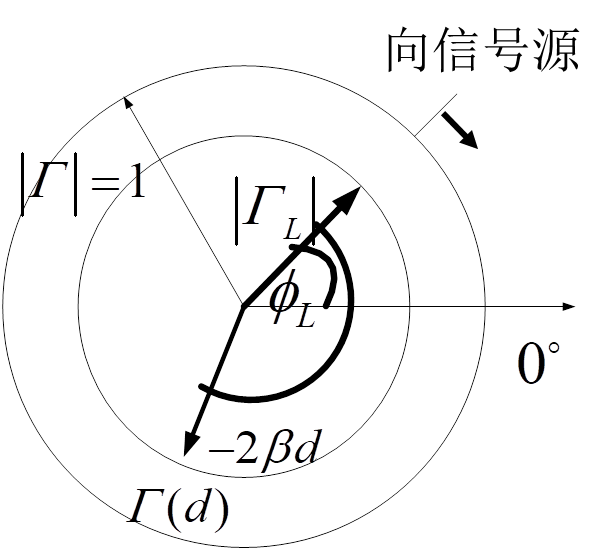
\includegraphics[width=4.5cm]{chart2.png}
    \end{column}
  \end{columns}
\end{frame}

\begin{frame}{反射参量}
  \begin{itemize}
    \item 阻抗与反射系数关系
  \end{itemize}
  \begin{align*}
    & V(d)=V^{+}(d)+V^{-}(d)=V^{+}(d)[1+\Gamma(d)]\\
    & I(d)=I^{+}(d)+I^{-}(d)=I^{+}(d)[1-\Gamma(d)]
  \end{align*}
  输入阻抗与反射系数间的关系
  \begin{empheq}[box=\widefbox]{align*}
    Z_{in}(d)=\frac{V^{+}(d)[1+\Gamma(d)]}{I^{+}(d)[1-\Gamma(d)]}=Z_{0}\frac{1+\Gamma(d)}{1-\Gamma(d)}
  \end{empheq}
\end{frame}

\begin{frame}{反射参量}
  \begin{empheq}[box=\widefbox]{align*}
    Z_{in}(d)=\frac{V^{+}(d)[1+\Gamma(d)]}{I^{+}(d)[1-\Gamma(d)]}=Z_{0}\frac{1+\Gamma(d)}{1-\Gamma(d)}
  \end{empheq}
  当传输线特性阻抗$Z_{0}$一定时,传输线上任意一点$d$处的阻抗$Z_{in}(d)$与该点的反射系数$\Gamma(d)$一一对应。可以通过测量反射系数获得传输线输入阻抗。\\
  \textbf{归一化}阻抗
  \begin{empheq}[box=\widefbox]{align*}
    z_{in}(d)=\frac{Z_{in}(d)}{Z_{0}}=\frac{1+\Gamma(d)}{1-\Gamma(d)}
  \end{empheq}
\end{frame}

\begin{frame}{反射参量}
  \begin{itemize}
    \item 传输系数$T$\qquad 描述传输线上的功率传输关系
  \end{itemize}
  \begin{columns}
    \begin{column}{0.5\linewidth}
      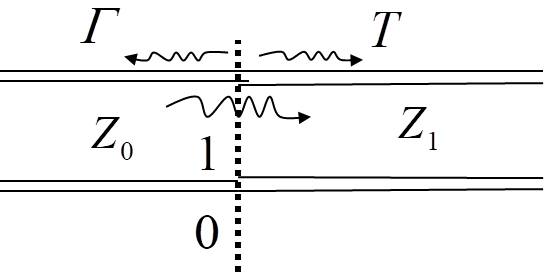
\includegraphics[width=4cm]{transPara.png}
    \end{column}
    \begin{column}{0.5\linewidth}
      \begin{align*}
        T=\frac{\text{传输电压或电流}}{\text{入射电压或电流}}=\frac{V^{t}}{V^{+}}=\frac{I^{t}}{I^{+}}
      \end{align*}
    \end{column}
  \end{columns}
  \begin{empheq}[box=\fbox]{align*}
    & V(z)=V^{+}_{0}(e^{-j\beta z}+\Gamma e^{j\beta z})\quad z<0\\
    & V(z)=V_{0}^{+}Te^{-j\beta z}\qquad\qquad\quad z>0
  \end{empheq}
  $Z=0$处两电压连续
  \begin{empheq}[box=\widefbox]{align*}
    T=1+\Gamma=1+\frac{Z_{1}-Z_{0}}{Z_{1}+Z_{0}}=\frac{2Z_{1}}{Z_{1}+Z_{0}}
  \end{empheq}
  插入损耗
  \begin{empheq}[box=\widefbox]{align*}
    L_{T}=-20\lg\lvert T \rvert \qquad (dB)
  \end{empheq}
\end{frame}

\begin{frame}{驻波参量}
  \begin{enumerate}
    \resume
    \item \textbf{驻波参量}
  \end{enumerate}
  \begin{itemize}
    \item 电压驻波比(VSWR)与行波系数K\\
    传输线上各点的电压和电流一般由入射波和反射波叠加而成,其结果在线上形成驻波,沿线各点的电压和电流的振幅不同,以$\lambda/2$周期变化。\\
    波腹点——振幅最大点\\
    波谷点——振幅最小点\qquad 波节点——振幅等于零的点\\
    \textbf{电压(或电流)驻波比VSWR}:定义为传输线上电压(或电流)振幅的最大值与最小值之比,或电压驻波系数$\rho$
    \begin{empheq}[box=\widefbox]{align*}
      VSWR=\rho=\frac{\lvert V\rvert_{max}}{\lvert V\rvert_{min}}=\frac{\lvert I\rvert_{max}}{\lvert I\rvert_{min}}
    \end{empheq}
  \end{itemize}
\end{frame}

\begin{frame}{驻波参量}
  \textbf{行波系数K}:定义为传输线上电压(或电流)的最小值与最大值之比,故行波系数与驻波比互为倒数。
  \begin{empheq}[box=\widefbox]{align*}
    K=\frac{1}{VSWR}=\frac{\lvert V\rvert_{min}}{\lvert V\rvert_{max}}=\frac{\lvert I\rvert_{min}}{\lvert I\rvert_{max}}
  \end{empheq}
\end{frame}

\begin{frame}{驻波参量}
  传输线任意点电压和电流
  \begin{align*}
    V(d)=V^{+}(d)[1+\lvert\Gamma_{L}\rvert e^{j(\Phi_{L}-2\beta d)}]\\
    I(d)=I^{+}(d)[1-\lvert\Gamma_{L}\rvert e^{j(\Phi_{L}-2\beta d)}]
  \end{align*}
  \begin{columns}
    \begin{column}{0.5\linewidth}
      当传输线上入射波与反射波同相叠加时,合成波出现最大值;而反向叠加时出现最小值。
    \end{column}
    \begin{column}{0.5\linewidth}
      \begin{align*}
        \lvert V(d)\rvert_{max}=v^{+}(d)[1+\lvert\Gamma_{L}\rvert]\\
        \lvert V(d)\rvert_{min}=v^{+}(d)[1-\lvert\Gamma_{L}\rvert]
      \end{align*}
    \end{column}
  \end{columns}
  驻波比与反射系数的关系式为:
  \begin{columns}
    \begin{column}{0.65\linewidth}
      \begin{empheq}[box=\widefbox]{align*}
        \rho=VSWR=\frac{\lvert V\rvert_{max}}{\lvert V\rvert_{min}}=\frac{1+\lvert\Gamma_{L}\rvert}{1-\lvert\Gamma_{L}\rvert}
      \end{empheq}
    \end{column}
    \begin{column}{0.35\linewidth}
      \begin{empheq}[box=\widefbox]{align*}
        \lvert\Gamma_{L}\rvert=\frac{\rho-1}{\rho+1}
      \end{empheq}
    \end{column}
  \end{columns}
\end{frame}

\begin{frame}{驻波参量}{沿线阻抗分布}
  线上任一点处的输入阻抗为:
  \begin{align*}
    Z_{in}(z)=Z_{0}\frac{Z_{L}+jZ_{0}\tan\beta z}{Z_{0}+jZ_{L}\tan\beta z}=R_{in}(z)+jX_{in}(z)
  \end{align*}
  (1)阻抗的数值周期性变化,在电压的波腹点和波谷点,阻抗分别为最大值和最小值
  \begin{align*}
    Z_{in}(波腹)=\frac{\lvert U\rvert_{max}}{\lvert I\rvert_{min}}=Z_{0}\frac{1+\lvert\Gamma\rvert}{1-\lvert\Gamma\rvert}=Z_{0}\rho\qquad \text{开路}\\
    Z_{in}(波谷)=\frac{\lvert U\rvert_{min}}{\lvert I\rvert_{max}}=Z_{0}\frac{1-\lvert\Gamma\rvert}{1+\lvert\Gamma\rvert}=Z_{0}\rho\qquad \text{短路}
  \end{align*}
  (2)每隔$\lambda/4$,阻抗性质变换一次;每隔$\lambda/2$,阻抗值重复一次。
\end{frame}

\begin{frame}{驻波参量}
  \begin{itemize}
    \item 阻抗与驻波参量的系数
  \end{itemize}
  由分布参数阻抗
  \begin{empheq}[box=\widefbox]{align*}
    Z_{in}(d)=Z_{0}\frac{Z_{L}+jZ_{0}\tan\beta d}{Z_{0}+jZ_{L}\tan\beta d}
  \end{empheq}
  \centering
  $\downarrow$
  \begin{empheq}[box=\widefbox]{align*}
    Z_{L}=Z_{0}\frac{Z_{in}(d)-jZ_{0}\tan\beta d}{Z_{0}-jZ_{in}(d)\tan\beta d}
  \end{empheq}
  \begin{columns}
    \begin{column}{0.6\linewidth}
      选取驻波最小点为测量点——距离负载的第一个电压驻波最小点位置
    \end{column}
    \begin{column}{0.4\linewidth}
      \begin{align*}
        Z_{in}(d_{min})=Z_{0}/VSWR=Z_{0}/\rho
      \end{align*}
    \end{column}
  \end{columns}
  \flushleft
  终端短路,确定电压波节点作参考点,接上负载测量参考点附近电压驻波最小点。
  \begin{columns}
    \begin{column}{0.5\linewidth}
      \begin{empheq}[box=\fbox]{align*}
        Z_{L}=Z_{0}\frac{1-j\rho\tan\beta d_{min}}{\rho-j\tan\beta d_{min}}
      \end{empheq}
    \end{column}
    \begin{column}{0.5\linewidth}
      负载阻抗和驻波参量一一对应
    \end{column}
  \end{columns}
\end{frame}

\subsection{无耗线工作状态分析}
\begin{frame}{无耗线工作状态}
  任何传输线上的电压函数只可能是入射波和反射波的迭加(构成Standing Wave)。不同传输线的区别仅仅在于入射波和反射波的成分不同。换句话说,通解是完备的,我们不需要再找,也不可能再找到其他解。\\
  边界条件确定$A_{1}$和$A_{2}$。边界条件的求取过程中,也孕育着一种思想,即网络思想(Network Idea):已知输入求输出;或已知输出求输入。
\end{frame}

\begin{frame}{无耗线工作状态}
  \begin{empheq}[box=\widefbox]{align*}
    V(z)=A_{1}e^{-j\beta z}+A_{2}e^{+j\beta z}
  \end{empheq}
  \begin{empheq}[box=\widefbox]{align*}
    V(d) & =\frac{1}{2}(V_{L}+Z_{0}I_{L})e^{j\beta d}+\frac{1}{2}(V_{L}-Z_{0}I_{L})e^{-j\beta d}\\
    & =V^{+}(d)+V^{-}(d)
  \end{empheq}
  \begin{empheq}[box=\widefbox]{align*}
    I(z)=\frac{1}{Z_{0}}(A_{1}e^{-j\beta z}+A_{2}e^{+j\beta z})
  \end{empheq}
  \begin{empheq}[box=\widefbox]{align*}
    I(d) & =\frac{1}{2Z_{0}}(V_{L}+Z_{0}I_{L})e^{j\beta d}-\frac{1}{2Z_{0}}(V_{L}-Z_{0}I_{L})e^{-j\beta d}\\
    & =I^{+}(d)+I^{-}(d)
  \end{empheq}
\end{frame}

\begin{frame}{无耗线工作状态}
  \begin{itemize}
    \item 传输线上反射波的大小,可用反射系数的模、驻波比和行波系数三个参量来描述。\\
    \begin{columns}
      \begin{column}{0.5\linewidth}
        反射系数模的变化范围为\\
        驻波比的变化范围为\\
        行波系数的变化范围为
      \end{column}
      \begin{column}{0.3\linewidth}
        \fbox{$0\leq\lvert\Gamma\rvert\leq 1$}\\
        \fbox{$1\leq\rho\leq\infty$}\\
        \fbox{$0\leq K\leq 1$}
      \end{column}
    \end{columns}
    \item 传输线的工作状态一般分为三种:\\
    (1)行波状态 \qquad $\lvert\Gamma\rvert=0,\rho=1,K=1$ \\
    (2)行驻波状态\quad $0<\lvert\Gamma\rvert<1 \quad 1<\rho<\infty \quad 0<K<1$\\
    (3)驻波状态 \qquad $\lvert\Gamma\rvert=1 \quad \rho=\infty \quad K=0$
  \end{itemize}
\end{frame}

\begin{frame}{无耗线工作状态}
  \begin{enumerate}
    \item \textbf{行波状态(无反射情况)}
    \begin{columns}
      \begin{column}{0.4\linewidth}
        条件:\\
        $Z_{L}=Z_{0}\rightarrow$\\
        $\Gamma_{L}=0,\rho=1,K=1$
      \end{column}
      \begin{column}{0.6\linewidth}
        \begin{empheq}[box=\widefbox]{align*}
          \Gamma_{L}=\frac{A_{2}}{A_{1}}=\frac{Z_{L}-Z_{0}}{Z_{L}+Z_{0}}\\
          =\left\lvert\frac{Z_{L}-Z_{0}}{Z_{L}+Z_{0}}\right\rvert e^{j\Phi_{L}}=\lvert\Gamma_{L}\rvert e^{j\Phi_{L}}
        \end{empheq}
      \end{column}
    \end{columns}
    由始端条件解
    \begin{empheq}[box=\widefbox]{align*}
      V(z)=\frac{V_{0}+I_{0}Z_{0}}{2}e^{-j\beta z}=V_{0}^{+}e^{-j\beta z}\\
      I(z)=\frac{V_{0}+I_{0}Z_{0}}{2Z_{0}}e^{-j\beta z}=I_{0}^{+}e^{-j\beta z}
    \end{empheq}
    \saveenum
  \end{enumerate}
\end{frame}

\begin{frame}{无耗线工作状态}
  \begin{columns}
    \begin{column}{0.5\linewidth}
      \begin{empheq}[box=\widefbox]{align*}
        v(z,t)=\lvert V_{0}^{+}\rvert\cos(\omega t-\phi_{0}-\beta z)\\
        i(z,t)=\lvert I_{0}^{+}\rvert\cos(\omega t-\phi_{0}-\beta z)
      \end{empheq}
      $\phi_{0}$为初相角,行波状态下的分布规律:\\
      (1)线上电压和电流的振幅恒定不变\\
      (2)电压行波与电流行波同相,它们的相位是位置$z$和时间$t$的函数,$v(z,t)$和$i(z,t)$初相均为$\phi_{0}$,因为$Z_{0}$是实数\\
      (3)线上的输入阻抗处处相等,且均等于特性阻抗
    \end{column}
    \begin{column}{0.5\linewidth}
      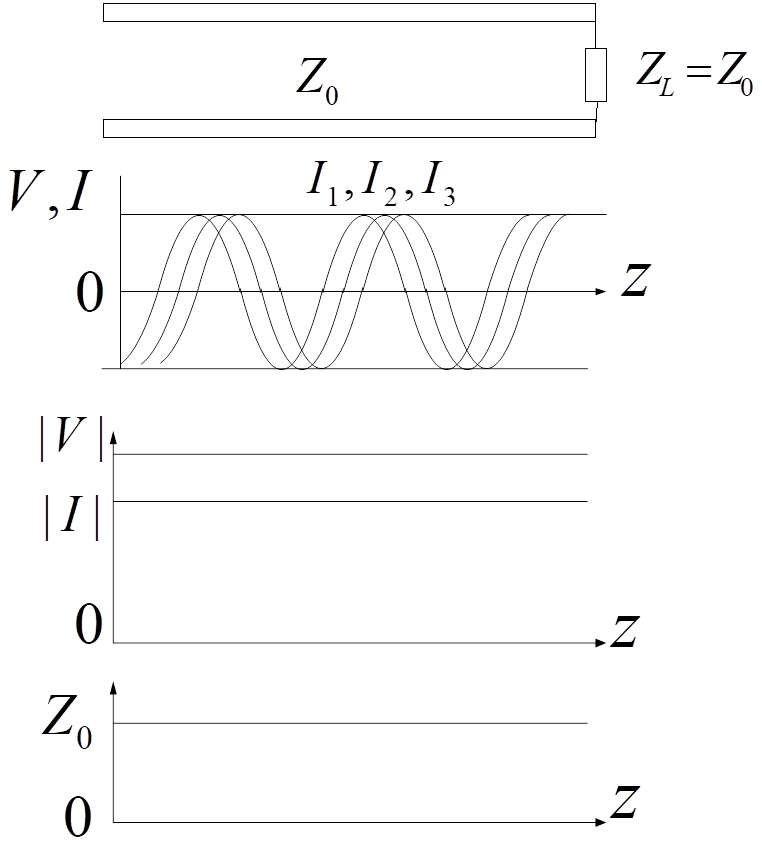
\includegraphics[width=5cm]{xingbo.png}
    \end{column}
  \end{columns}
\end{frame}

\begin{frame}{无耗线工作状态}
  \begin{enumerate}
    \resume
    \item \textbf{驻波状态(全反射情况)}
    \saveenum
  \end{enumerate}
  反射系数模等于1的全反射情况称为驻波状态。
  \begin{empheq}[box=\widefbox]{align*}
    \Gamma_{L}=\frac{A_{2}}{A_{1}}=\frac{Z_{L}-Z_{0}}{Z_{L}+Z_{0}}=\left\lvert\frac{Z_{L}-Z_{0}}{Z_{L}+Z_{0}}\right\rvert e^{j\phi_{L}}=\lvert\Gamma_{L}\rvert e^{j\phi_{L}}
  \end{empheq}
  条件:终端短路;终端开路;终端接纯电抗负载\\
  \qquad \quad$Z_{L}=0$,\qquad$Z_{L}=\infty$,\qquad$Z_{L}=\pm jX_{L}$\\
  终端的入射波将被全反射,沿线入射波与反射波迭加形成驻波分布。驻波状态意味着入射波功率一点也没有被负载吸收,即\textbf{负载与传输线完全失配}。
\end{frame}

\begin{frame}{无耗线工作状态}
  \begin{itemize}
    \item 终端短路
  \end{itemize}
  \begin{empheq}[box=\widefbox]{align*}
    Z_{L}=0,\Gamma_{L}=\frac{Z_{L}-Z_{0}}{Z_{L}+Z_{0}}=-1\rightarrow VSWR=\frac{1+\lvert\Gamma_{L}\rvert}{1-\lvert\Gamma_{L}\rvert}=\infty
  \end{empheq}
  \begin{align*}
    V(d)&=V^{+}(d)+V^{-}(d)=V_{L}^{+}(e^{j\beta d}-e^{-j\beta d})=j2V_{L}^{+}\sin\beta d\\
    I(d)&=I^{+}(d)+I^{-}(d)=I_{L}^{+}(e^{j\beta d}+e^{-j\beta d})=2I_{L}^{+}\cos\beta d\\
    &=\frac{2V_{L}^{+}}{Z_{0}}\cos\beta d
  \end{align*}
  短路时的驻波状态分布规律:\\
  (1)瞬时电压或电流在传输线的某个固定位置上随时间$t$作正弦或余弦变化,而在某一时刻随位置$d(z)$也作正弦或余弦变化,但瞬时电压和电流的时间相位差和空间相位差均为$\pi/2$,这表明传输线上没有功率传输。
\end{frame}

\begin{frame}{无耗线工作状态}
  \only<1>{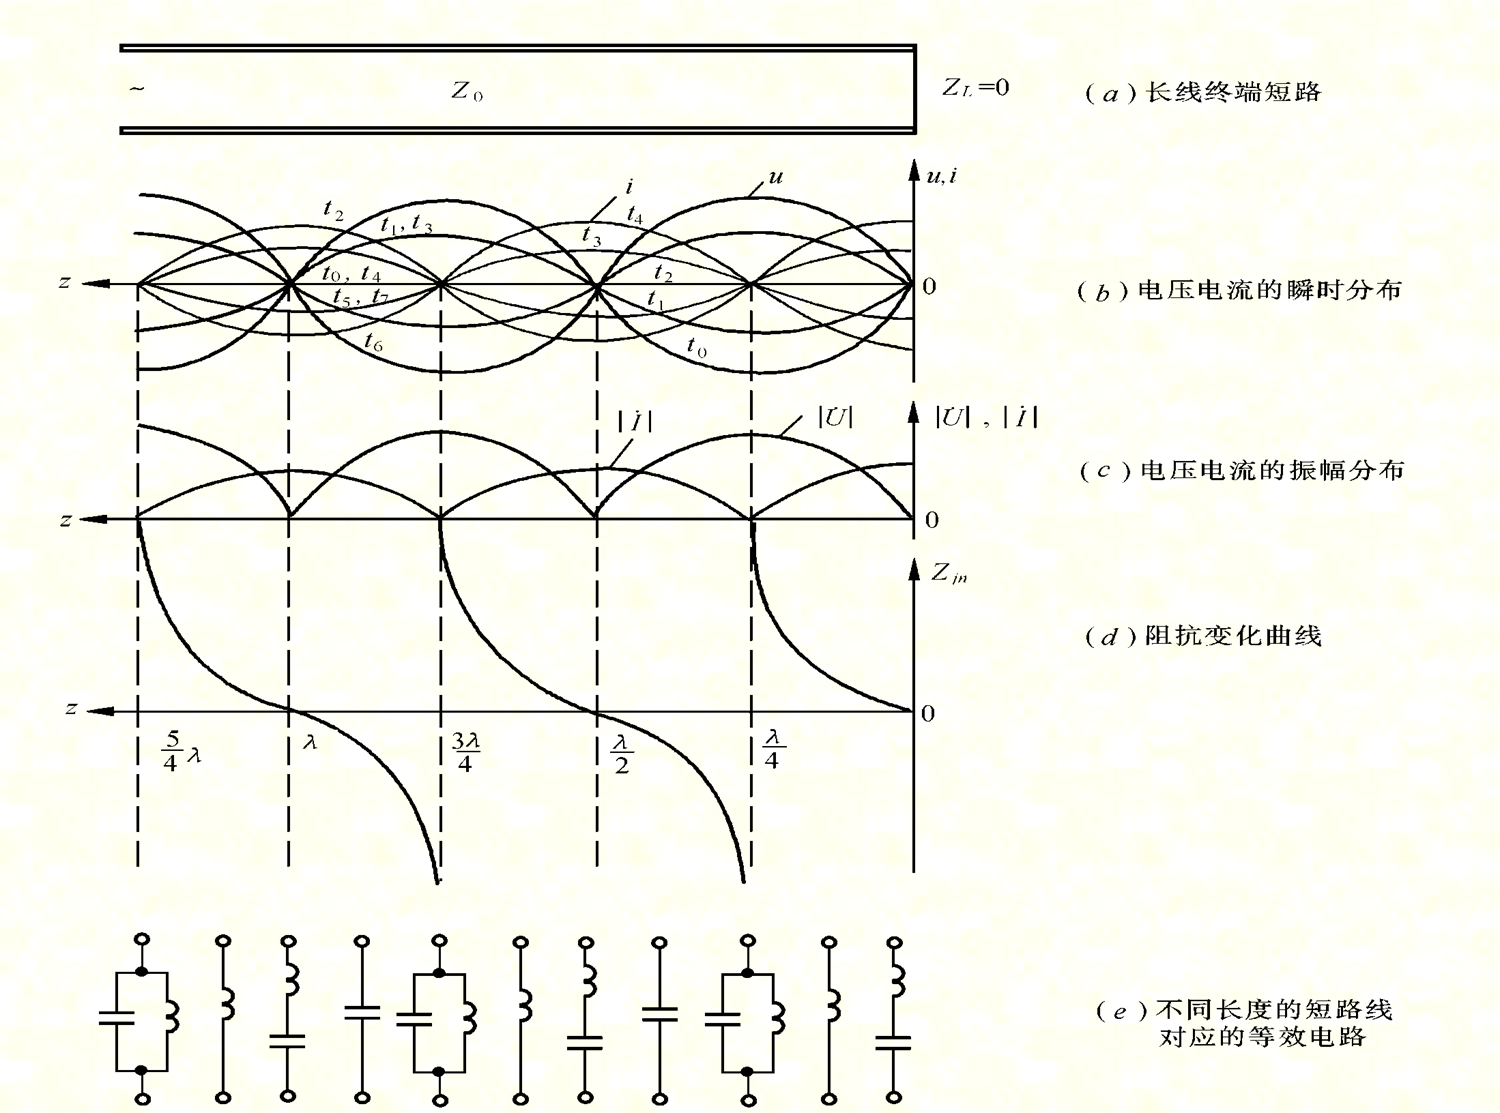
\includegraphics[width=10cm]{duanlu.png}}
  \only<2>{\begin{columns}
   \begin{column}{0.55\linewidth}
    \begin{empheq}[box=\widefbox]{align*}
     d=(2n+1)\lambda/4,(n=0,1,\ldots)\\
     \lvert V\rvert_{max}=2\lvert V_{L}^{+}\rvert
    \end{empheq}
    \begin{empheq}[box=\widefbox]{align*}
     d=n\lambda/2,(n=0,1,\ldots)\\
     \lvert V\rvert_{min}=0
    \end{empheq}
   \end{column}
   \begin{column}{0.45\linewidth}
    (2)电压振幅最大值,而电流振幅恒为零,这些点称之为电压的波腹点和电流的波节点;\\
    电流振幅恒为最大值,而电压振幅恒为零,这些点称之为电流的波腹点和电压的波节点。
   \end{column}
  \end{columns}}
  \only<3>{
  \begin{table}[h!]
    \begin{center}
      \caption{终端短路情况}
      \begin{tabular}{|c|c|}
        \hline
        $ \beta d=n\pi $ & $ \beta d=(2n+1)\pi/2 $ \\
        $ d=n\lambda/2 $ & $ d=(2n+1)\lambda/4 $ \\
        \hline
        $\text{电压节点}\lvert V(d)\rvert=0$ & $\text{电压腹点}\lvert V(d)\rvert=2\lvert V_{L}^{+}\rvert$ \\
        $\text{电流腹点}\lvert I(d)\rvert=2\lvert I_{L}^{+}\rvert$ &$ \text{电流节点}\lvert I(d)\rvert=0$ \\
        \hline
      \end{tabular}
    \end{center}
  \end{table}
  }
  \only<4>{(3)传输线终端短路时,输入阻抗为纯电抗。\\
  \begin{empheq}[box=\widefbox]{align*}
    Z_{in}^{sc}(d)=Z_{0}\frac{Z_{L}+jZ_{0}\tan\beta d}{Z_{0}+jZ_{L}\tan\beta d}=jZ_{0}\tan\beta d=jZ_{0}\tan\frac{2\pi d}{\lambda}=jX_{in}
  \end{empheq}}
\end{frame}

\begin{frame}{无耗线工作状态}
  \begin{itemize}
    \item 终端开路
  \end{itemize}
  \begin{empheq}[box=\widefbox]{align*}
    Z_{L}=\infty,\Gamma_{L}=\frac{Z_{L}-Z_{0}}{Z_{L}+Z_{0}}=1\rightarrow VSWR=\frac{1+\lvert\Gamma_{L}\rvert}{1-\lvert\Gamma_{L}\rvert}=\infty
  \end{empheq}
  \begin{align*}
    &\Gamma_{L}=V_{L}^{-}/V_{L}^{+}=1 \quad V_{L}^{-}=V_{L}^{+}\\
    &V(d)=V^{+}(d)+V^{-}(d)=2V_{L}^{+}\cos\beta d\\
    &I(d)=I^{+}(d)+I^{-}(d)=j2I_{L}^{+}\sin\beta d\\
    &Z_{in}^{oc}(d)=-jZ_{0}\cot\beta d
  \end{align*}
  \begin{columns}
    \begin{column}{0.5\linewidth}
      终端短路
      \begin{empheq}[box=\widefbox]{align*}
        Z_{L}=0,\Gamma_{L}=-1\rightarrow VSWR=\infty
      \end{empheq}
    \end{column}
    \begin{column}{0.5\linewidth}
      \begin{empheq}[box=\widefbox]{align*}
        & V(d)=j2V_{L}^{+}\sin\beta d\\
        & I(d)=2I_{L}^{+}\cos\beta d\\
        & Z_{in}^{sc}(d)=jZ_{0}\tan\beta d
      \end{empheq}
    \end{column}
  \end{columns}
\end{frame}

\begin{frame}{无耗线工作状态}
  (1)负载处,或\fbox{$d=n\lambda/2,(n=0,1,\ldots)$}\\
  电流$I_{L}=0$为电流波节点,\\
  电压为最大值$V_{L}=2V_{L}^{+}$为电压波腹点
  \begin{table}[h!]
    \begin{center}
      \caption{终端开路情况}
      \begin{tabular}{|c|c|}
        \hline
        $\beta d=n\pi$ & $\beta d=(2n+1)\pi/2$ \\
        $d=n\lambda/2$ & $d=(2n+1)\lambda/4$\\
        \hline
        电压腹点$\lvert V(d)\rvert=2\lvert V_{L}^{+}\rvert$ & 电压节点$\lvert V(d)=0\rvert$ \\
        电流节点$\lvert I(d)=0\rvert$ & 电流腹点$\lvert I(d)\rvert=2\lvert I_{L}^{+}\rvert$ \\
        \hline
      \end{tabular}
    \end{center}
  \end{table}
  (2)输入阻抗\\
  $Z_{in}^{oc}(d)=-jZ_{0}\cot\beta d\Longleftrightarrow$ 短路 \fbox{$Z_{in}^{sc}=jZ_{0}\tan\beta d$}\\
  经过观察:\textbf{把开路线可以看成是短路线移动$\lambda/4$而成}
\end{frame}

\begin{frame}{无耗线工作状态}
  \begin{columns}
    \begin{column}{0.5\linewidth}
      短路状态
      \begin{empheq}[box=\widefbox]{align*}
        & V(d)=j2V_{L}^{+}\sin\beta d\\
        & I(d)=2I_{L}^{+}\cos\beta d
      \end{empheq}
      \begin{empheq}[box=\widefbox]{align*}
        Z(d)=jZ_{0}\tan\beta d
      \end{empheq}
      作$d'=d+\lambda/4,V_{L}^{+}=j\tilde V_{L}^{+}$变换,即可由开路线转化为短路线。不能疏忽了$V_{L}^{+}=j\tilde V_{L}^{+}$的条件,长度$d'$移动条件只对$\lvert V_{L}^{+}\rvert$和阻抗有效,\textbf{相位}是不等价的。
    \end{column}
    \begin{column}{0.5\linewidth}
      开路状态
      \begin{empheq}[box=\widefbox]{align*}
        & V(d)=2V_{L}^{+}\cos\beta d\\
        & I(d)=j2I_{L}^{+}\sin\beta d
      \end{empheq}
      \centering
      $\Downarrow$
      \begin{empheq}[box=\widefbox]{align*}
        & V(d')=j2\tilde V_{L}^{+}\sin\beta d'\\
        & I(d')=2\tilde I_{L}^{+}\cos\beta d'
      \end{empheq}
      \begin{empheq}[box=\widefbox]{align*}
        Z(d)=-jZ_{0}\cot\beta d
      \end{empheq}
      $\Downarrow$
      \begin{empheq}[box=\widefbox]{align*}
        Z(d')=jZ_{0}\tan\beta d'
      \end{empheq}
    \end{column}
  \end{columns}
\end{frame}

\begin{frame}{无耗线工作状态}
  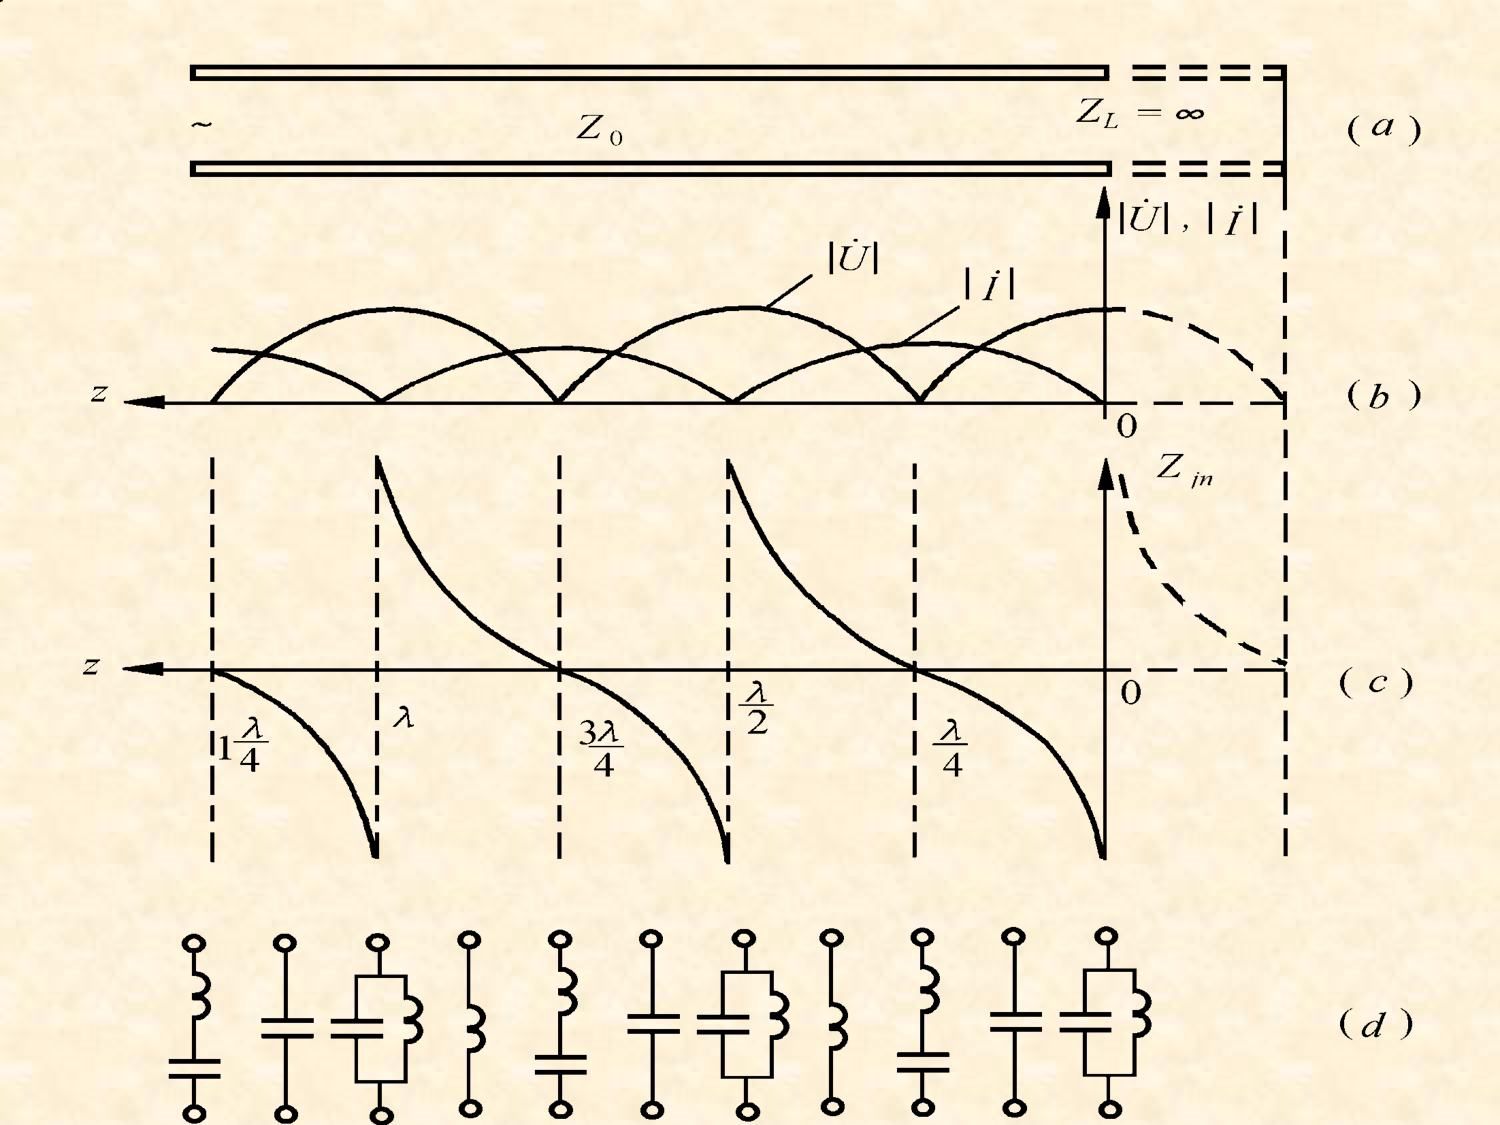
\includegraphics[width=10cm]{kailu.png}
\end{frame}

\begin{frame}{无耗线工作状态}
  \begin{align*}
    Z_{in}^{oc}(d)=-jZ_{0}\cot\beta d \qquad Z_{in}^{sc}(d)=jZ_{0}\tan\beta d\\
    Z_{in}^{oc}(d)\cdot Z_{in}^{sc}(d)=Z_{0}^{2}
  \end{align*}
  \begin{itemize}
    \item 对于一定长度$d$的传输线,通过开路和短路的测量,可以得到如下参数:
  \end{itemize}
  \begin{align*}
    &Z_{0}=\sqrt{Z_{in}^{oc}(d)\cdot Z_{in}^{sc}(d)}\\
    &\beta=\frac{1}{d}\arctan\sqrt{\frac{Z_{in}^{sc}(d)}{Z_{in}^{oc}(d)}}
  \end{align*}
\end{frame}

\subsection{有耗线的特性与计算}
\begin{frame}{有耗线的特性与计算}

\end{frame}

\subsection{Smith Chart(阻抗圆图及其应用)}
\begin{frame}{Smith Chart(阻抗圆图及其应用)}

\end{frame}

\subsection{传输线的阻抗匹配}
\begin{frame}{传输线的阻抗匹配}

\end{frame}
